\section{Results \& Outlook}
\label{sec:outro}

The project's goals of interactively creating bifurcation diagrams using Galerkin's method and continuation methods could be met.
There are some further points of interest for similar or following projects of this type.

On a practical level, one of the things an implementation of the sort of this project might benefit from are Broyden updates.
In its basic form, the method allows to update the Jacobian of the system of equations obtained from the Galerkin operator.
Though calculating the Jacobian is a time-consuming task, this is of minor interest, as the effort is negligible compared to the effort for inverting the Jacobian, which is needed for each computation of the tangent.

One of the main sources of complications are orbits which change their direction too fast.
As is the case in the Rössler system for high values of $c$ and in the Lorenz System for low values of $\rho$. %pics
In these regions the optimization procedure converges slowly and the predictor-corrector method's step-size adaption suggests very small steps (as seen from the bifurcation view).
This is likely caused by choosing a truncated Fourier series as a model for the solution candidates.
Ringing effects as in the Gibbs phenomenon support this thesis.
This kind of model is, though natural for periodic functions, not a natural choice for sharp turning functions.
No attempts were made to investigate the definite reason for this behavior, however, choosing a model which is better adapted to these challenges might allow for more accurate results in these areas.
Furthermore, solution branches could be traced further, as these effects are a cause of stopping the tracing of solutions in the Rössler, as well as in the Lorenz system. %ref
In the case of the Rössler system this is less of a problem, as the solutions for high $c$ did not appear to reveal anything of immediate interest.
However, in the Lorenz system the behavior prohibited tracing the solutions in the $\rho < 20$ area.
It is this area, where there is a huge amount of interaction between the branches of solutions.

Modeling the trajectories as linear combinations of non-equidistant B-splines instead of complex oscillations might yield interesting results. %cite
\begin{itemize}
	\item The periodicity requirement can be enforced by choosing the basis vectors appropriately.
	\item Through adaption of the knots, the degree of smoothness can be varied to the point being $C^0$ only.
		This can be done by changing \emph{multiplicities} of knots, that is, by having several knots be equal.
		An interesting point is that this change in continuity can occur dynamically through optimizing the knot vector.
	\item Spline curves can easily be differentiated.
	\item Adding and removing control-points is possible.
		This might allow for dynamic adaption of a solution candidate, if necessary.
\end{itemize}
Chances are good, that candidate solutions modeled this way can be fit into a framework similar to the one above while at the same time gaining the ability to do non-differentiable turns.

%\begin{figure}[!h]
	%\centering
	%\makebox[0pt]{
		%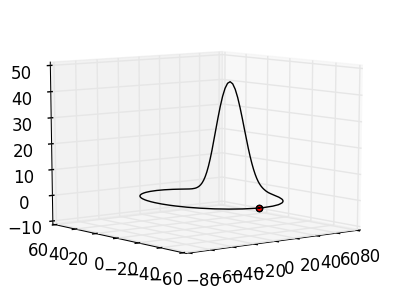
\includegraphics[scale=.5]{img/1.png}
		%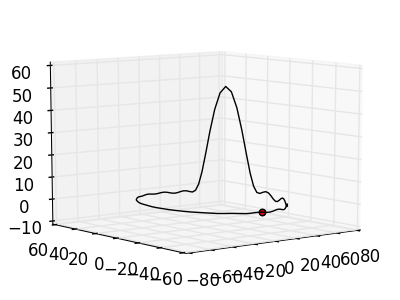
\includegraphics[scale=.5]{img/2.png}
		%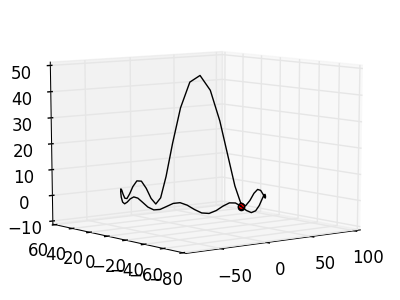
\includegraphics[scale=.5]{img/3.png}
	%}
	%\caption{A periodic orbit in the Rössler modeled by a decreasing number of coefficients, illustrating the ringing effect.}
	%\label{fig:end}
%\end{figure}